\section{Introduction}

Software platforms diversity and hardware heterogeneity, as discussed in Chapter \ref{chap:background}, constitutes a major obstacle for software testing. In fact, running tests requires many environment configurations and settings in order to test the whole application. For example, testing a web application requires the installation of the maven dependencies, web server, libraries, etc. When software developers upgrades the web server version for example, they need to rebuild the application and run the same integration tests in order to check that no errors  have been incorporated. Thus, testing applications using different execution environments and system settings becomes very time consuming and tedious.

For instance, as we discussed in Chapter \ref{chap:code generators} and \ref{chap:compilers}, to evaluate the automatically generated code (by either code generators or compilers), we use to generate code, compile it, and then run test cases. To do so, different system configurations were required to ensure these steps such as installing the generator version (GCC or Haxe versions), install interpreters, compilers, maven dependencies, etc. 

One way to test these configurable generators is to use the virtualization technology. For instance, an alternative method leverages container-based system virtualization (\eg, Docker, as discussed in Section \ref{sec:Lightweight system virtualization for software testing}) to automate the code generation, deployment, and testing inside pre-configured software containers.
This technology enables to mimic the execution environment settings and reproduce the tests in isolated and highly configurable system containers.

When it comes to evaluate the resource consumptions of automatically generated code, this technology becomes very valuable because it allows a fine-grained resource management and isolation. Moreover, it facilitates resource usage extraction and limitation of programs running inside containers. 

This chapter presents a technical description of this lightweight runtime environment and its benefit for automating the non-functional testing of generated code. This infrastructure is used in our two first contributions as means to run tests in a configurable execution environment and to efficiently collect resource consumption metrics.

This chapter is organized as follows: 

Section \ref{mon:System containers} introduces system containers as a lightweight execution environment. We show the benefit of using this technology to automate software testing.

Section \ref{mon:Runtime Testing} describes the runtime monitoring components required to collect resource usage metrics.

Section \ref{mon:case study} shows the adaptation of this sandboxing infrastructure to the generator case study as it is used in Chapters \ref{chap:code generators} and \ref{chap:compilers}.

Finally, we conclude in Section \ref{mon:coclusion}.


\section{System containers as a lightweight execution environment}
\label{mon:System containers}
System containers are operating system-level virtualization method that allows running multiple isolated Linux systems on a control host using a single Linux kernel. 
Containers share the same OS and hardware as the hosting machine and it is very useful to use them in order to create new configurable and isolated instances to run. 
Container-based virtualization reduces the overhead associated with having each guest running a new installed operating system such the case for virtual machines. This approach can also improve the performance because there is just one operating system taking care of hardware calls.
The Linux kernel provides the control groups\footnote{\url{https://fr.wikipedia.org/wiki/Cgroups}} (Cgroups) functionality that allows the limitation and prioritization of resources (CPU, memory, block I/O, network, etc.) inside containers so that, one container does not starve the others in terms of resources.
%Thus, it provides ways to control how much memory, CPU, or block IO a container can use. 

For instance, Docker\footnote{\url{https://www.docker.com}} is a popular container-based technology that automates the deployment of any application as a lightweight, portable, and self-sufficient container, running virtually on a host machine~\cite{merkel2014docker}. 
Today, Docker is one of the most popular infrastructure technology adopted in cloud computing\cite{peinl2016docker}. 
For example, in 2015, Docker had about 3\% market share, and by 2017 it is running on 15\% of the hosts\footnote{\url{https://www.datadoghq.com/docker-adoption/}}.
%To achieve that, Docker uses the Linux container technology. 
Using Docker, it is possible to define pre-configured applications and servers to host as virtual images. It also defines the way the service should be deployed in the host machine using configuration files called Dockerfiles. Moreover, we can enable some configuration options to control and limit resources. For example, we can provide option flags to limit how much memory or CPU usage each service is allowed to consume, associate CPU cores to each service, etc. 


In short, the main advantages of this micro-services approach are:
\begin{itemize}
	\item The use of containers induces less performance overhead compared to using a full stack virtualization solution~\cite{spoiala2016performance}. Indeed, instrumentation and monitoring tools for memory profiling like Valgrind~\cite{nethercote2007valgrind} can induce too much overhead.
	\item Thanks to the use of Dockerfiles, it is possible to easily configure the execution environment in order to build and customize applications using numerous settings (\eg, generator version, dependencies, host IP and OS, optimization options, etc.). Thus, we can use the same configured Docker image to execute different instances of the same application. For hardware architecture, containers share the same platform architecture as the host machine (\eg, x86, x64, ARM, etc.). 
	\item Docker uses Linux control groups (Cgroups) to group processes running in the container. This allows us to manage the resources of a group of processes, which is very valuable. 
	This approach increases the flexibility when we want to manage resources, since we can manage every group individually. For example, if we would evaluate the non-functional requirements of generated code within a resource-constraint environment, we can  request and limit resources within the execution container according to the needs.
	\item Although containers run in isolation, they can share data with the host machine and other running containers. Thus, non-functional data relative to resource consumption can be gathered and managed by other containers (\ie, for storage purpose, visualization)
\end{itemize}

%Thus, instead of configuring all code generators under test (GUTs) within the same host machine, we wrap each GUT within a system container. Afterwards, a new instance of the container is created to enable the execution of generated code in an isolated and configured environment. Meanwhile, we start our runtime testing components. A monitoring component collects usage statistics of all running containers and save them at runtime in a time series database component. Thus, we can compare later information about the resource usage of generated programs and detect inconsistencies within code generators.


%For this purpose, we propose a testing infrastructure based on System Container techniques such as Docker\footnote{\url{https://www.docker.com}} environment. 
%This framework automates the deployment and execution of applications inside software containers by allowing multiple program configurations to run autonomously on different servers (i. e., a cloud servers).
%It also provides a distributed environment where system storage and resources can be finely managed and limited according to the needs. 

%Thus, we integrate a collection of components to define the adequate infrastructure for testing and monitoring of code generators. 






\section{Runtime Monitoring Engine}
\label{mon:Runtime Testing}
In order to monitor the applications (\ie, tests) running within containers, we aim to use a set of Docker components to ease the extraction of resource usage information.


\subsection{Monitoring Container}
First, a monitoring component is needed to collect the resource usage and performance characteristics of running containers. As discussed earlier, Docker relies on Cgroups file systems to expose a lot of metrics about accumulated CPU cycles, memory, block I/O usage, etc. Therefore, our monitoring component automates the extraction of these runtime performance metrics stored in Cgroups files. 
Among the popular ways to do that is to monitor each container via the Docker API, or by installing an agent for detailed visibility inside each container. 
The Docker client already provides a command-line tool to inspect containers' resource consumption. The command \textit{docker stats}, for example, can be used to get the stats about the running containers at runtime. 
If we want to do that manually, we can access to live resource consumption of each container available at the Cgroups file system via stats found in \textit{``/sys/fs/cgroup/cpu/docker/(longid)/''} (for CPU consumption) and \textit{``/sys/fs/cgroup/memory/docker/(longid)/''} (for stats related to memory consumption). Our monitoring component automates the process of service discovery and metrics aggregation for each new container. Thus, instead of gathering manually metrics located in Cgroups file systems, it extracts automatically the runtime resource usage statistics relative to the running component (\ie, the executed test suite within a container). We note that resource usage information is collected in raw data. This process may induce a little overhead because it performs a very fine-grained accounting of resource usage on running container. Fortunately, this may not affect the gathered data since we run only one test suite or application within each container.
To ease the monitoring process, we integrate cAdvisor, a Container Advisor\footnote{\url{https://github.com/google/cadvisor}}. cAdvisor monitors service containers at runtime as described above. It has been widely used in different projects such as Heapster\footnote{\url{https://github.com/kubernetes/heapster}} and Google Cloud Platform\footnote{\url{https://cloud.google.com/}}. 

However, cAdvisor monitors and aggregates live data over only 60 seconds interval. Therefore, we record all data over time, since container's creation, in a time-series database. It allows the end users to run queries and define non-functional metrics from historical data. Thereby, to make the gathered data truly valuable for resource usage monitoring, we link our monitoring component to a back-end database container. 



\subsection{Back-end Database Container}
This component represents a time-series database back-end. It is plugged with the previously described monitoring component to save the non-functional data for long-term retention, analytics and visualization. 
During application execution, resource usage stats are continuously sent to this component. When a container is killed, we are able to access to its relative resource usage metrics through the database. We choose a time series database because we are collecting time series data that correspond to the resource utilization profiles of programs execution.

We use InfluxDB\footnote{\url{https://github.com/influxdata/influxdb}}, an open source distributed time-series database as a back-end to record data. InfluxDB allows the user to execute SQL-like queries on the database. For example, the following query reports the maximum memory usage of container \textit{``generated\_code\_v1''} since its creation:

\begin{lstlisting}[
language=SQL,
showspaces=false,
basicstyle=\small,
numberstyle=\small,
commentstyle=\color{gray},
linewidth=\columnwidth
]
select max (memory_usage) from stats 
where container_name='generated_code_v1'
\end{lstlisting}
\label{listing}

To give an idea about the data gathered by the monitoring component and stored in the time-series database, we describe in Table \ref{tab:metrics} these collected metrics:
\begin{table}[h]
	\begin{center}
			\resizebox{0.6\columnwidth}{!}{%
		\begin{tabular}{|p{1.4cm}|p{7.6cm}|}
			\hline
			\textbf{Metric} & \textbf{Description} \\
				\hline
			Name & Container Name \\\hline
			
			T & Elapsed time since container's creation \\\hline
			
			Network  &  Stats for network bytes and packets\\\hline
			
			Disk IO &  Disk I/O stats \\\hline
			
			Memory  &  Memory usage \\\hline
			
			CPU &  CPU usage \\
			\hline
			
		\end{tabular}%
	}
		
	\end{center}
	\caption {Resource usage metrics recorded in InfluxDB}
	\label{tab:metrics}
\end{table}

Apart from that, we provide information about the application size (\eg, size of generated binaries) and the compilation time required to produce code.
For instance, resource usage statistics are collected and stored using the previously described components. It is relevant to show resource usage profiles of running programs overtime. To do so, we present a front-end visualization container for resource usage profiling. 

\subsection{Front-end Visualization Container}

Once we gather and store resource usage data, the next step is visualizing them. That is the role of the visualization container. It will be the endpoint component that we use to visualize the recorded data. Therefore, we provide a dashboard to run queries and view different resource consumption profiles of running components, through a Web UI. Thereby, we can compare visually the profiles of resource consumption among containers. Moreover, we can use this component to export the data currently being viewed into static CSV document. So, we can perform statistical analysis on this data to detect inconsistencies or performance anomalies.
As a visualization component, we use Grafana\footnote{\url{https://github.com/grafana/grafana}}, a time-series visualization tool available for Docker. Grafana lets us display live results over time in much pretty looking graphs. Same as InfluxDB, we use SQL queries to extract the non-functional data from the database for visualization and analysis.

\section{The generator case study}
\label{mon:case study}
We present now an adaptation of this micro-service infrastructure to the generator case study, as applied in Chapters \ref{chap:code generators} and \ref{chap:compilers}. We recall that we used containers as means for running different variants of optimized code in Chapter \ref{chap:compilers}, and for running a bench of test suites across different software platforms in Chapter \ref{chap:code generators}. 
The runtime monitoring components, presented in this chapter, are used in both contributions to evaluate the resource usage of generated code. 
An overview of the micro-service and technical solutions applied for the generator case study are shown in Figure \ref{mon:infra}. In the following, we describe in details the infrastructure settings. The experimental material is also available online\footnote{\url{https://testingcodegenerators.wordpress.com/}}\footnote{\url{https://noticegcc.wordpress.com/}}.

\begin{figure}[h]
	\centering
	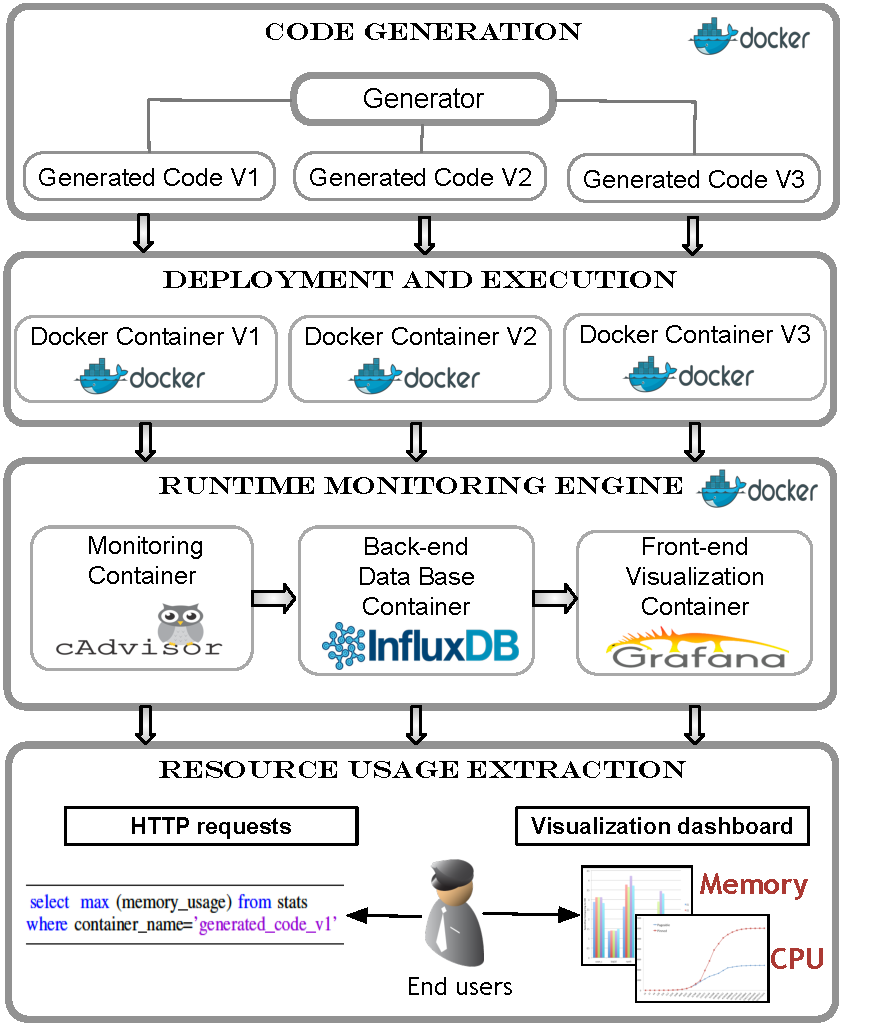
\includegraphics[width=0.73\linewidth]{chapitre5/fig/infra_summary}
	\caption{Our container-based infrastructure for automatic generators testing}
	\label{mon:infra}
\end{figure}


\paragraph{Code generation}
Before starting to monitor and test applications, we have to deploy the generated code (by compilers or code generators) on different Docker containers. 
Thus, instead of configuring all generators under test (GUTs) within the same host machine, we deploy each GUT within a container. To do so, we create a new configuration image for each GUT (\ie, the Docker image) where we install all the libraries, compilers, and dependencies needed to ensure the code generation and compilation. Thereby, the GUT produces code within multiple instances of pre-configured Docker images. So, we use Dockerfiles to configure all these settings.
We use the public Docker registry\footnote{\url{https://hub.docker.com/}} (a cloud-based registry service) to save and manage all our Docker images. 
Once code generation is done, the generated output files are saved in a shared repository. In Docker environment, this repository is called \textit{data volume}. It is a specially-designated directory within containers that shares data with the host machine and with other running containers.
 
\paragraph{Deployment and execution}
Next, generated code (in the \textit{data volume}) is executed individually inside an isolated Docker container. By doing so, we ensure that each executed program runs in isolation without being affected by the host machine or any other processes. Moreover, since a container is cheap to create, we are able to create too many containers as long as we have new programs to execute (\eg, new optimized code, test suite for a specific software platform, etc.).
Since each program execution requires a new container to be created, it is crucial to remove and kill containers that have finished their job to eliminate the load on the system. We run the experiment on top of a private data-center that provides a bare-metal installation of Docker. On a single machine, containers are running sequentially and we pin $p$ cores and $n$ Gbytes of memory for each container\footnote{$p$ and $n$ can be cofigured}. Once the execution is done, resources reserved for the container are automatically released to enable spawning next containers. Therefore, the host machine will not suffer too much from performance trade-offs.

\paragraph{Runtime monitoring}
While running containers, we run the three monitoring containers described above in order to monitor the running workload. To do so, we use Docker Compose\footnote{\url{https://docs.docker.com/compose/overview/}} to run all containers simultaneously. The concept of Docker Compose is similiar to Dockerfiles. It uses a configuration file to run and link multi-container Docker services. We set up the Compose file so that we run all services and particularly to map running containers to cAdvisor and InfluxDB, using Docker ports and network links in order to stream resource usage data.

\paragraph{Resource usage extraction}
The end users have two ways to extract the information about the resource usage of generated code. It is possible to directly request the remote time series database via HTTP requests, executing SQL-like queries like the example presented in Section \ref{listing}. They can request different metrics such as CPU, memory usage, disk writing speed, etc. An alternative solution is to visualize the resource consumption of generated code within the web-based dashboard provided by Grafana. The visualization tool is not used when auto-tuning and testing generators because we just needed to extract the CPU or memory usage for each test or optimized code. 

We use the same hardware across all experiments in Chapters \ref{chap:code generators} and \ref{chap:compilers}: an AMD A10-7700K APU Radeon(TM) R7 Graphics processor with 4 CPU cores (2.0 GHz), running Linux with a 64 bit kernel and 16 GB of system memory. 


\begin{remark}
	We would notice that this testing infrastructure can be generalized and adapted to other case studies other than generators. Using system containers, any software application/generated code can be easily deployed within containers (\ie, by configuring the container image). It will be later executed and monitored using our runtime monitoring engine. 
\end{remark}

\section{Conclusion}
\label{mon:coclusion}
We presented in this chapter, the technical details of the infrastructure used to collect the non-functional metrics (e.g., memory and CPU consumptions) of automatically generated code (by either compilers or code generators). This solution offers effective support for automatically deploying, executing, and testing the generated code in different environment settings.
The same monitoring infrastructure is used to evaluate quality of generated code in the two first contributions of this thesis. The experiments conducted in Chapters \ref{chap:code generators} and \ref{chap:compilers} showed the usefulness of this infrastructure for tuning and testing generators.